% !TEX program = xelatex
% !TEX root = main.tex
\documentclass[black,normal,cn,hide]{elegantbook}

\usepackage{pdflscape}
\usepackage{tabu}
\usepackage{booktabs} 
\usepackage{colortbl} 
\usepackage{xcolor} 
\usepackage{xfrac}
\usepackage{tikz}
\usepackage{titling}
\usepackage{bytefield}
\usepackage{longtable}
\usepackage{graphicx}
\usepackage{float} 
\usepackage{cite}
\renewcommand\maketitlehooka{\null\mbox{}\vfill}
\renewcommand\maketitlehookd{\vfill\null}

\newcommand{\artdate}{2022年8月}
\newcommand{\artauthor}{陈泱宇,李燕琴}
\newcommand{\arttitle}{CDIM 决赛设计报告}
\newcommand{\todo}{\textbf{\textcolor{red}{此部分尚需完善。}}}
\newcommand{\hlrule}{\rule{\linewidth}{0.5mm}}

\pagestyle{fancy}
\fancyhf{}
\rhead{\thepage}
\lhead{\arttitle}
\cfoot{\thepage}

\begin{document}

% \begin{titlepage}
%     \vspace*{\fill}
%     \begin{center}
%         \rule{\linewidth}{0.2 mm} \\[0.4 cm]
%         { \huge \bfseries \thetitle}\\
%         \rule{\linewidth}{0.2 mm} \\[1.5 cm]
%         \vspace*{2cm}
%         \includegraphics[scale = 0.618]{logo.jpg}\\[1.0 cm]
%     \end{center}
%     \vspace*{\fill}
% \end{titlepage}

\begin{titlepage}
    % \rule{\linewidth}{0.5mm}
    \vfill
    \center 
    \textit{\Large “龙芯杯”第六届全国大学生计算机系统能力培养大赛}\\[0.5cm] 
    \texttt{\Large 重庆大学 “所以延迟槽会消失对不队”队}
  
    \vspace{1.5 cm}
    \hlrule \\[0.4 cm]
    { \huge \bfseries CDIM 项目}\\[0.4cm]
    { \huge \bfseries 决赛设计报告}\\
    \hlrule \\[1cm]
   
    \begin{figure}[h]
      \centering
      \includegraphics[width=0.5\linewidth]{img/logo.png}
    \end{figure}
   
   \vspace{0.5 cm}
  
    \vspace{.5 cm}
    陈泱宇\\
    cyy@cyyself.name\\
    \vspace{.5 cm}
    李燕琴\\
    maxpicca@qq.com\\
    \vspace{.5 cm}
    王梓宇\\
    925136384@qq.com\\
    \vspace{.5 cm}
    张翀\\
    20194159@cqu.edu.cn\\
  
    \vspace{2 cm}
    {\large \artdate}\\[3cm] 
  
  \vfill
  
\end{titlepage}

\tableofcontents
\mainmatter

% 可以使用input(但是无法显示outline),或直接在正文写
\chapter{概述}

\section{项目背景}
本项目依托于龙芯杯提供的FPGA实验平台、Soc工程环境以及基准测试程序,设计并实现了一个部分兼容 MIPS32 体系结构的小端序 CPU,名为CDIM(\textbf{C}QU \textbf{D}ual \textbf{I}ssue \textbf{M}achine),其能成功通过龙芯杯提供的功能测试、性能测试、系统测试,具有较完善的运算处理、AXI访问、异常处理、中断响应等功能,并能够运行u-boot引导程序、uCore操作系统和Linux操作系统等。

\section{名词解释}
本项目中可能用到的一些名词缩写及其解释如表\ref{table:abbreviation_definition}所示。

\begin{table}[!htbp]
    \centering
    \caption{名词缩写和解释}
    \label{table:abbreviation_definition}
    
    \begin{tabular}{cll}
    \toprule
    \multicolumn{1}{c}{\textbf{名词缩写}} & \multicolumn{1}{c}{\textbf{全称}}                   & \multicolumn{1}{c}{\textbf{解释}} \\ 
    \midrule
    MIPS                               & Microprocessor without Interlocked Pipeline Stages & 无内部互锁流水级的微处理器                \\
    SOC                                & System On a Chip                                   & 片上系统                             \\
    MIPS                               & Microprocessor without Interlocked Pipeline Stages & 无内部互锁流水级的微处理器 \\
    SOC                                & System On a Chip                                   & 片上系统 \\
    CPU                                & Central Processing Unit                            & 中央处理器 \\
    ALU                                & Arithmetic Logic Unit                              & 算数逻辑单元 \\
    GPR                                & General Purpose Register                           & 通用寄存器 \\
    CP0                                & Co-Processor 0                                     & 协处理器0 \\
    BRAM                               & Block Random Access Memory                         & 块随机访问存储器 \\
    FIFO                               & First In First Out                                 & 先进先出 \\
    RAW                                & Read After Write                                   & 写后读 \\
    WAW                                & Write After Write                                  & 写后写 \\
    WAR                                & Write After Read                                   & 读后写 \\
    \bottomrule
    \end{tabular}
\end{table}

\section{项目概述}
CDIM(\textbf{C}QU \textbf{D}ual \textbf{I}ssue \textbf{M}achine),采用对称双发射五级顺序流水线的设计,支持指令FIFO、分支预测、指令缓存和数据缓存等特殊单元,以提升系统性能。其中双发射,采用对称双发逻辑以充分保证双发率;五级顺序流水线由取指(Instruction Fetch)、译码(Instruction Decode)、执行(Excute)、访存(Memory access),写回(Write Back)五个阶段组成;指令FIFO可以隔离取指阶段和后续阶段,以实现高效取指的作用;指令缓存和数据缓存均采用二路组相联和突发传输的设计,单路均为4KB以匹配TLB页面要求,其中指令缓存一行为64bit以适应双发取指要求,数据缓存一行为32bit。\todo 此外,CDIM还支持U-Boot引导程序,并基于该引导程序,成功运行uCoreh和Linux操作系统。
% TODO: 系统运行这一段陈述



\newpage
\renewcommand{\bibname}{参考文献}
\begin{thebibliography}{99}
	\bibitem[1]{MIPS} MIPS® Architecture For Programmers I, II, III. Imagination Technologies LTD.  
\end{thebibliography}



\end{document}